%!TEX root=thesis.tex
\chapter{Automating Radio Cross-identification}
\label{cha:cross-identification}

  In this chapter, we develop a machine learning approach to the radio
  cross-identification problem.

  We first need to formalise the radio cross-identification problem in a machine
  learning context. This is the focus of Section
  \ref{sec:cross-identification-formalism}, where we cast the problem as an
  object localisation problem that can be solved with standard classification
  methods. Section \ref{sec:features} discusses how we can represent galaxies as
  vectors for classification, and Section \ref{sec:binary-classifiers}
  investigates which classification method should be used for this task.

  We will also need some benchmark to test our methods against; our
  approach to evaluation of methods without groundtruth is discussed in Section
  \ref{sec:norris-as-groundtruth}. We describe our experimental design in
  Section \ref{sec:experiment-design}.

  As the Radio Galaxy Zoo label set is sourced from volunteers, we wish to
  investigate some of the many methods for dealing with crowdsourced labels.
  This is the focus of Section \ref{sec:rgz-crowd-labels}, where we look at
  applying majority vote and the \citeauthor{raykar10} method to the Radio
  Galaxy Zoo label set.

  In Section \ref{sec:rgz-results} we train our classifiers on expert labels and
  on the Radio Galaxy Zoo and compare the results. Finally, in Section
  \ref{sec:cross-identification-conclusion-future-work}, we conclude and suggest
  some avenues for future work.

\section{Formalism}
\label{sec:cross-identification-formalism}

  We begin by restating the cross-identification problem (Section
  \ref{sec:radio-cross-identification}). When we look at the sky with radio
  telescopes, we see the radio emissions from the jets of AGNs. Given an image
  of these radio emissions, and possibly other images in other wavelengths, we
  want to locate the host galaxy containing the associated AGN. In general,
  there may be multiple hosts associated with one radio object (such as in
  Figure \ref{fig:two-hosts}), but we make the assumption that there is only
  one. This greatly simplifies the problem.

  \begin{figure}
    \centering
    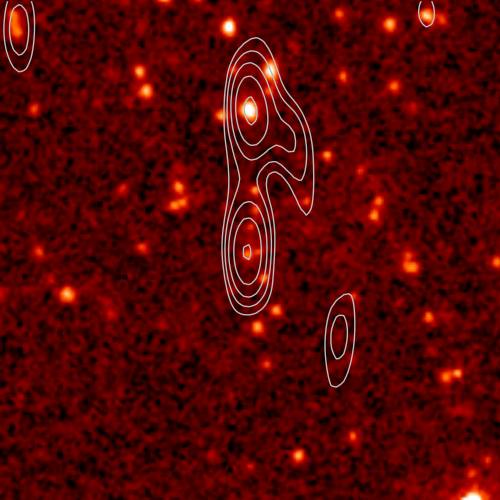
\includegraphics[width=0.5\textwidth]{images/CI0370C1_heatmap+contours.png}
    \caption{A radio object (ARG0003ra1) with two host galaxies. This radio
      object is actually two radio objects that have been incorrectly detected
      as one, and there is one host galaxy for each object.}
    \label{fig:two-hosts}
  \end{figure}

  \subsection{Cross-identification as Object Localisation}
  \label{sec:object-localisation}

    We can interpret cross-identification as an object localisation problem. As
    input, we have an image of the radio sky, and we want to locate a host
    galaxy in this image. A common way to find an object in an image is by using
    a sliding window. A fixed-size image patch centred on each pixel is taken as
    a representation of that pixel. This is then used as input to a
    classification model which outputs a probability for each pixel, with higher
    probabilities corresponding to higher likelihood of the object being located
    at that pixel. The pixel with the highest probability is considered the
    location of the object.

    This may be slow depending on the size of the image. One way to improve upon
    this approach is to first identify a small number of candidate locations,
    and then only examine patches around these locations. For the cross-%
    identification problem, we can use galaxy locations as candidate pixels,
    with galaxies found in infrared surveys such as WISE and SWIRE.
    Additionally, astronomical measurements such as magnitude are included in
    these surveys and these may be taken as additional features for each
    candidate pixel, giving more information to the classifier.

  \subsection{The Galaxy Classification Task}
  \label{sec:galaxy-classification-task}

    This approach can be formalised as follows. Consider a set $\mathcal X$ of
    candidate host galaxies, and a radio object $r$ that we want to assign a
    host galaxy. Let $y : \mathcal X \to \{0, 1\}$ represent whether a given $x
    \in \mathcal X$ is the host galaxy associated with $r$. Under the assumption
    that a radio object has exactly one associated host galaxy, then there
    exists exactly one $x \in \mathcal X$ such that $y(x) = 1$, and for all
    other $x \in \mathcal X$, $y(x) = 0$. The cross-identification task then
    amounts to modelling $p(y(x) = 1 \mid x, r)$. Once this distribution is
    modelled, the host galaxy associated with $r$ is given by
    \begin{equation}
        \label{eq:cross-identification}
        \mbox{host}(r) = \underset{x}{\mbox{argmax}}\ p(y(x) = 1 \mid x, r).
    \end{equation}

    Ideally, $\mathcal X$ is the set of all galaxies. This is clearly
    intractable, so as an approximation we use a catalogue of infrared objects
    near the radio object of interest, taken from an infrared survey. We also
    make the assumption that the host galaxy is within $1'$ of the radio object
    --- while this doesn't hold in general, systems larger than $1'$ are rare
    and require human insight to discover \citep{banfield16}.

\section{Evaluating Performance Without Groundtruth}
  \label{sec:norris-as-groundtruth}

  In general, we do not have groundtruth for the cross-identification problem.
  While the groundtruth exists (a galaxy either has an AGN or does not), it is
  impossible for us to measure this accurately. Even expert catalogues, such as
  those provided by \citeauthor{norris06} (Section \ref{sec:norris}), are noisy
  --- \citep{norris06} estimate that their cross-identifications have a $9.02\%$
  false positive rate.
  
  Our primary source of labels for the classification task is the Radio Galaxy
  Zoo. These labels have been provided by non-experts, and as such are even more
  noisy. This leads to two problems: A classifier trained on the noisy labels
  may be inaccurate, and evaluating the performance of a trained classifier
  against noisy labels will not accurately reflect the true performance of the
  classifier. We address the former in Section \ref{sec:rgz-crowd-labels}, and
  the latter here.

  A straightforward way to evaluate classifier performance without groundtruth
  is to aggregate the Radio Galaxy Zoo crowd labels in some way to approximate
  the groundtruth, and then use that for evaluation. While there are many ways
  that we could aggregate the labels (Section \ref{sec:rgz-crowd-labels}), these
  aggregates are \emph{not} the groundtruth and may still contain high noise. We
  want our classifier to be capable of finding the best approximation to the
  groundtruth, not to the noisy inputs, and evaluation should reflect that. We
  therefore cannot use aggregated crowd labels for evaluation.

  To attempt to mitigate this problem, we combined the \citeauthor{norris06}
  catalogue (Section \ref{sec:norris}) with the \citeauthor{fan15} catalogue
  (Section \ref{sec:fan}) to obtain a test set with as little noise as possible.
  Each galaxy identified as hosting an AGN in the catalogues was matched to the
  nearest WISE or SWIRE object. Each matched object was then labelled $1$. All
  other galaxies in the infrared survey were labelled $0$. This produced two
  label sets, which we refer to as the \citeauthor{norris06} labels and the
  \citeauthor{fan15} labels respectively. We then took the intersection of these
  label sets to find a set of galaxies for which the label sets agree. Test sets
  were drawn only from this set of galaxies. This results in a test set where
  test instances are ``easier'' than a test set drawn from the entire data set,
  but any tests performed against these test sets should be more reliable than
  would otherwise be the case.

\section{Experiment Design}
\label{sec:experiment-design}

  To guide our classifier design, we needed to run experiments. This section
  describes the design and test sets used for the experiments that appear in the
  following sections.

  Note that in the experiments that follow later in this chapter, we have not
  used SWIRE. AllWISE is the infrared survey that EMU will be cross-identified
  with, and so we have chosen to focus on it.

  To generate the \citeauthor{norris06} and \citeauthor{fan15} label sets, we
  matched each location identified by \citeauthor{norris06} and
  \citeauthor{fan15} to the nearest candidate host in the AllWISE survey. These
  galaxies were labelled $1$. All other candidate hosts were labelled $0$.

  We generated test sets by first finding all candidate hosts for which the
  \citeauthor{norris06} label and the \citeauthor{fan15} label agree. To
  generate a test set, we followed the following method:
  \begin{enumerate}
    \item Find all ATLAS objects where \citeauthor{norris06} and
    \citeauthor{fan15} agree on the labels of all galaxies within 1'.
    \item Draw randomly without replacement 50\% of the ATLAS objects.
    \item If a candidate host is within 1' of a drawn ATLAS object, add it to
    the test set.
  \end{enumerate}
  This method resulted in a test set with similar class distribution to the true
  data and no feature overlap between training objects and testing objects. We
  drew 10 test sets with this method.

  To train and test a method, we followed the following method:
  \begin{enumerate}
    \item Choose a test set.
    \item Add all candidate hosts not in this test set to the training set.
    \item Train the method using the selected training set.
    \item Evaluate performance with balanced accuracy against the test set.
    \item Repeat for all other test sets.
  \end{enumerate}
  We report the mean balanced accuracy and standard deviation.

\section{Feature Selection}
\label{sec:features}

  To train a machine learning method to solve the galaxy classification task,
  we must find a representation of galaxies in a feature space $\mathbb{R}^D$.
  In this section we describe and motivate our choice of galaxy features,
  extracted from both infrared and radio surveys.

  \subsection{Infrared Features}
  \label{sec:ir-features}

    \begin{figure}
      \centering
      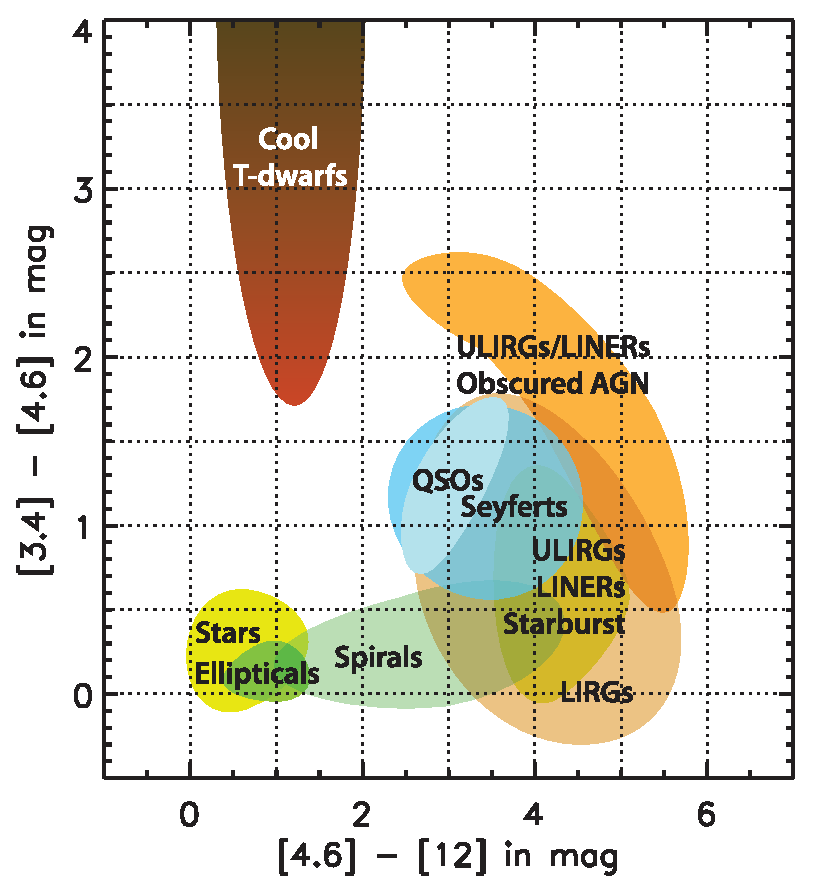
\includegraphics[width=0.5\textwidth]{images/wise_colour-colour}
      \caption{WISE colour-colour diagram showing the colours of various
        astronomical objects. The horizontal axis is $w2 - w3$ and the vertical
        axis is $w1 - w2$. \emph{Reproduced from \citet{wright10}.}}
      \label{fig:wise-colour-colour}
    \end{figure}

    As described in Section \ref{sec:cross-identification-formalism}, we need
    candidate host galaxies from an infrared catalogue. We have two choices here
    --- the WISE catalogue (Section \ref{sec:wise}) and the SWIRE catalogue
    (Section \ref{sec:swire}). WISE is lower resolution and less sensitive, but
    is the survey that will be used to cross-identify EMU (Section
    \ref{sec:emu}) sources when they are available. SWIRE has higher
    resolution and sensitivity, and thus would give more accurate galaxies, but
    it does not cover the whole sky. Here, we describe our choice of features
    for both.

    For WISE, we use all four WISE band magnitudes ($w1, w2, w3,$ and $w4$) as
    features. Since the features are magnitudes, they are on a logarithmic
    scale, and we found that in practice classification performance improved
    when the magnitudes were converted to their corresponding flux value. We
    performed this conversion with the formula
    \begin{equation}
      \label{eq:mag-to-flux}
      f = 10^{-0.4m}.
    \end{equation}
    This is the inverse of Equation \ref{eq:apparent-magnitude} with the flux in
    linear units of $f_{\text{Vega}}$ Jy.

    The ratios between infrared fluxes are indicators of physical galactic
    properties such as star formation and dust, and can be used to identify
    different classes of galaxies \citep{wright10}. In practice, the $w1 - w2$
    and $w2 - w3$ ratios are most commonly used (such as in Figure
    \ref{fig:wise-colour-colour}), so we chose to use these ratios as features.
    Once again, we used a linear scale, computing the ratios using equation
    \ref{eq:magnitude-difference} and converting them to linear units with
    Equation \ref{eq:mag-to-flux}.

    Also available were the unprocessed infrared images captured in the survey.
    Under the assumption that the large scale infrared structure of a galaxy is
    unchanged by an AGN, we ignored the images themselves and focused on
    features obtained from the catalogue. This greatly simplified feature
    selection with minimal expected impact on the classification performance.
    Future work may investigate the effectiveness of features extracted from
    infrared images on classification performance, but this is beyond the scope
    of this thesis.

    SWIRE also contains colour information, but unlike WISE, the information is
    in the form of fluxes instead of magnitudes. This means that the flux
    information in the catalogue can be used as features directly. The ratios
    can also be used as features: $3.6\ \mu\text{Jy} / 4.5\ \mu\text{Jy}$ and $4.5\
    \mu\text{Jy} / 5.8\ \mu\text{Jy}$ are the SWIRE equivalents of $w1 - w2$ and
    $w2 - w3$. Since SWIRE is higher resolution than WISE, the infrared images
    may contain more useful information and thus be useful for features, but
    this was not explored in this thesis.

    Both WISE and SWIRE catalogues contain the positions of each object. For the
    final infrared feature, we use the distance from an infrared object to the
    centre of the closest radio object.

  \subsection{Radio Features}
  \label{sec:radio-features}

    While the infrared catalogues include measurements on individual galaxies,
    the ATLAS radio catalogue does not. This is because galaxies are not visible
    in radio, so while galaxies are directly represented in an infrared
    catalogue they are not in a radio catalogue. Galactic features must thus be
    extracted from the radio images directly. We use a convolutional neural
    network for this purpose, as described in Section
    \ref{sec:image-feature-extraction}.

    We note that there is existing research on feature representations of radio
    galaxies. \citet{fan15} used an astronomical model of radio galaxies in
    ATLAS for cross-identification, and \citet{proctor06} investigated feature
    selection for radio galaxies in FIRST using hand-designed features. We do
    not use these methods here for two reasons: First, we wish to investigate
    automated feature extraction, and second, we wish to avoid dependence on any
    specific astronomical model. This is because we expect to find completely
    new objects in EMU that may not fit existing models, and machine learning
    algorithms like those we develop here will eventually be applied to EMU
    \citep{banfield15}.

    \subsubsection{Building a Model for Feature Extraction}
    \label{sec:feature-extraction-model}

      \begin{figure}
         \centering
         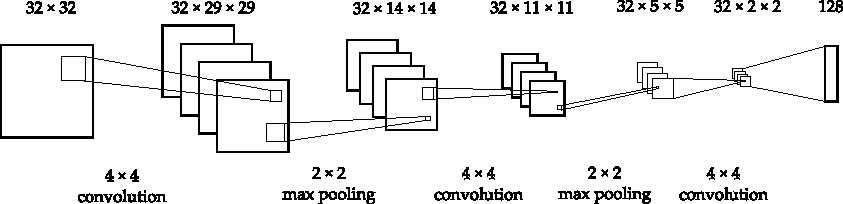
\includegraphics[width=\textwidth]{images/cnn_new.pdf}
         \caption{Convolutional neural network for radio feature extraction. The
           leftmost square represents the input image; the rightmost rectangle
           is the output.}
         \label{fig:radio-cnn}
       \end{figure}

      We chose to use a convolutional neural network (CNN) with three
      convolutional and max pooling layers, shown in Figure \ref{fig:radio-cnn}.
      This resulted in an 128-dimensional feature vector. For training this
      network, we added a 64-dimensional dense layer mapping to a 1-dimensional
      output. 10\% of ATLAS objects were selected at random and reserved for
      training the CNN, to ensure later testing data would not overlap the
      training set. The entire network was then trained to match the consensus
      Radio Galaxy Zoo labels of the galaxies nearest the reserved training set.

      A better approach would be to use a convolutional autoencoder, which would
      allow training on all the radio data, and data with no labels at all, but
      this was computationally infeasible for this project.

      An example of the neural network applied to a radio image is shown in
      Figure \ref{fig:rgz-cnn}.

      \begin{figure}
        \centering
        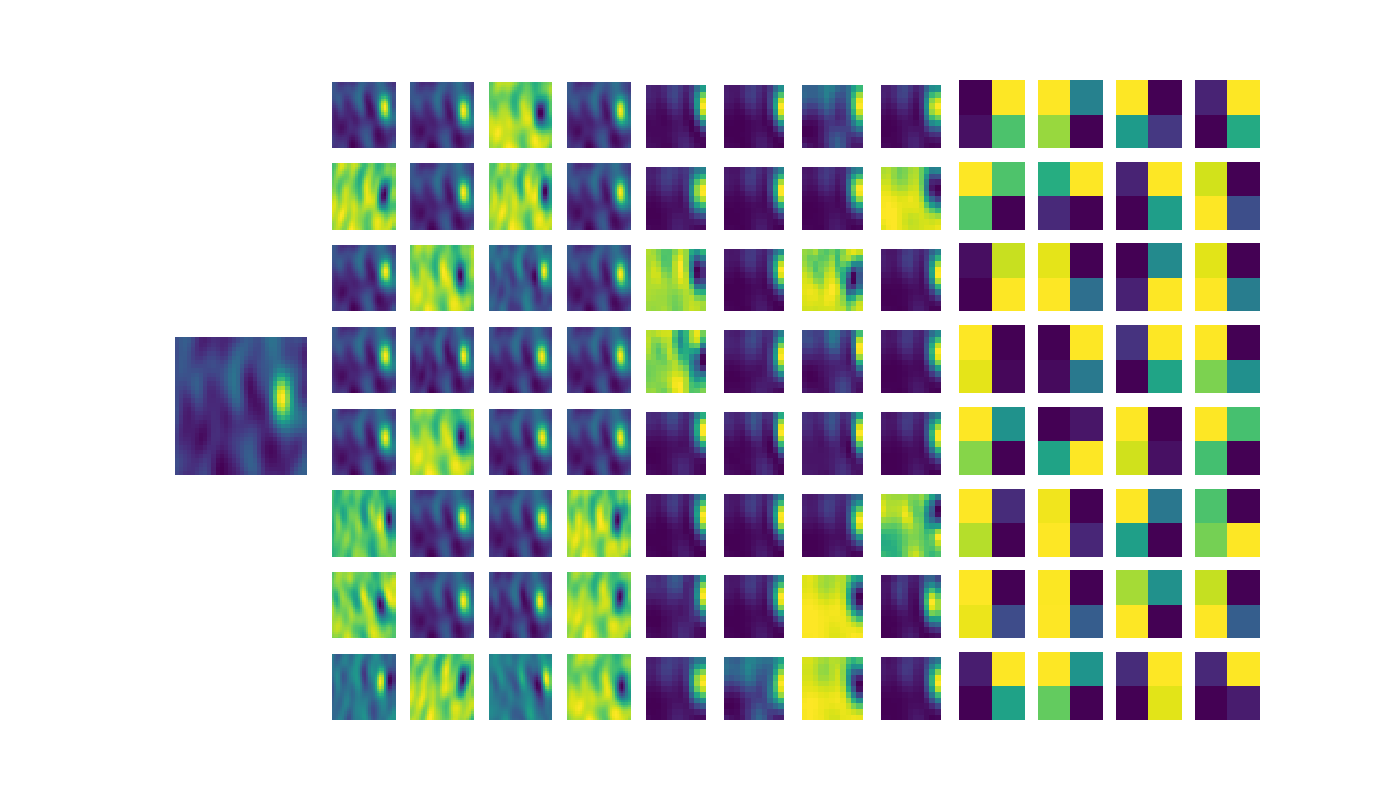
\includegraphics[width=\textwidth]{images/rgz_cnn}
        \caption{The effects of convolutional layers on an input image. The
          left-most image is the original radio image. The other images are the
          32 images output from each of the three convolutional layers.}
        \label{fig:rgz-cnn}
      \end{figure}

  \subsection{Feature Analysis}
  \label{sec:feature-analysis}

    To determine the effect of each set of features on classification
    performance, we performed a feature ablation experiment. We trained a
    logistic regression classifier on the \citeauthor{norris06} label set, each
    time using a different subset of features. The lower the resulting balanced
    accuracy, the more important the held out features. This was repeated ten
    times with different $50\%$ subsets of the training set. When holding out
    the WISE magnitude features, we also held out the CNN features, since we
    found that the CNN features tended to dominate results. These results are
    plotted in Figure \ref{fig:feature-ablation} and the means and standard
    deviations of the balanced accuracies can be found in Table
    \ref{tab:feature-ablation}. It is clear that the features extracted from the
    radio image are by far the most useful features; removing them causes the
    balanced accuracy to drop by $17.07 \pm 1.88$ percentage points. It also
    seems that some features, such as distance and $w1 - w2$, can act as
    distractors, though they may be useful features on their own. The inability
    of our classifier to ignore these features may be due to our use of $L2$
    regularisation.

    \begin{figure}
      \centering
      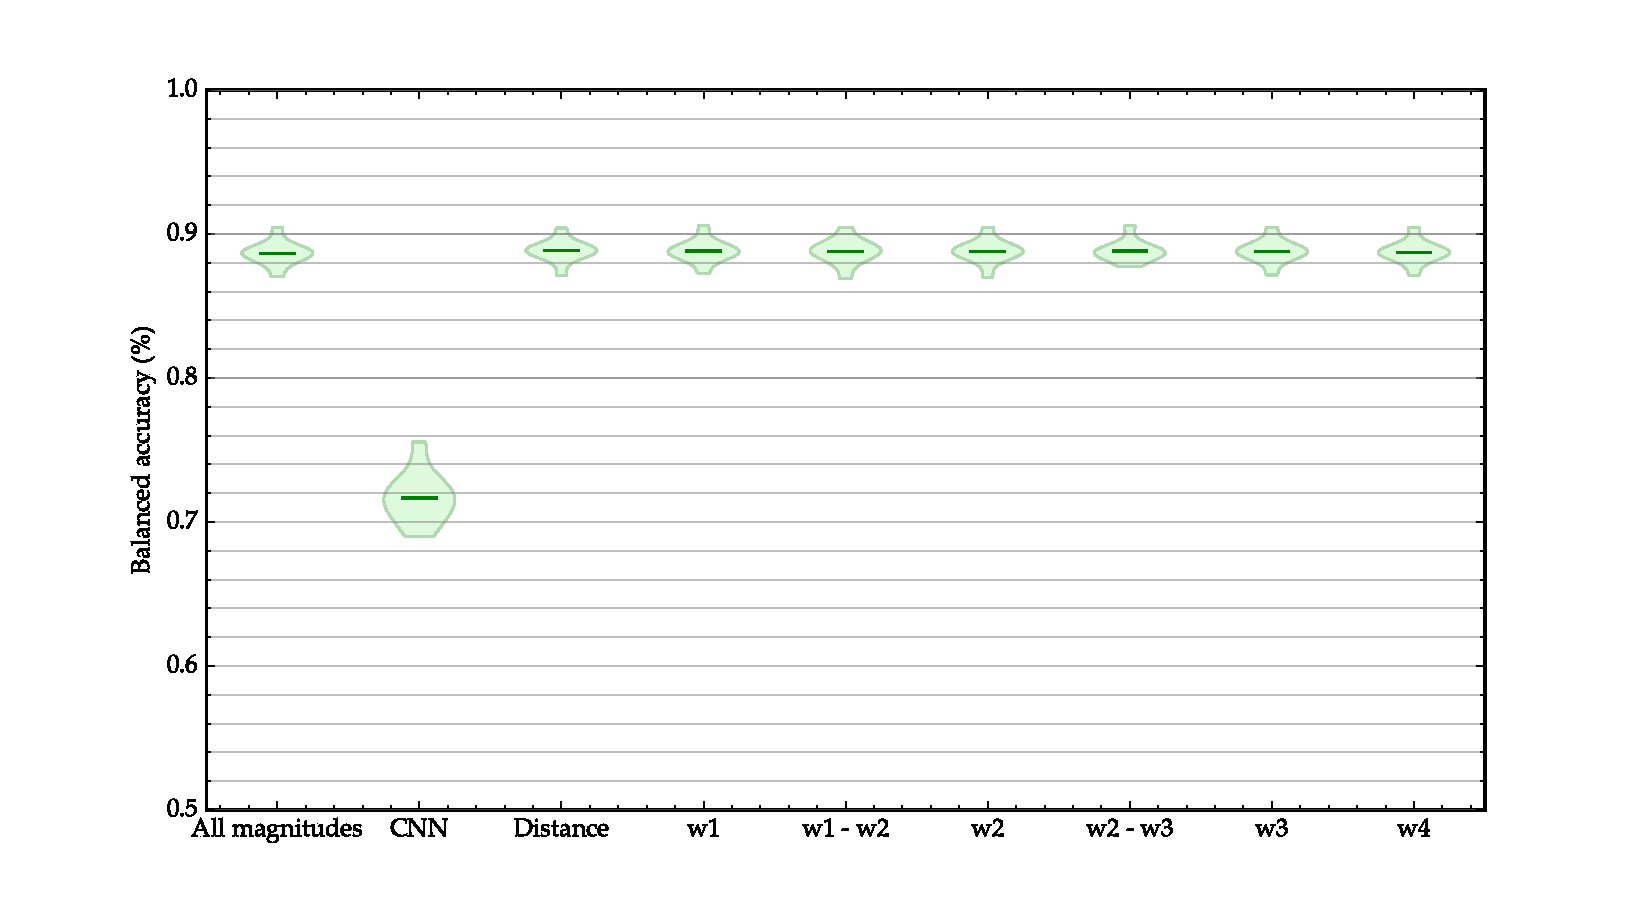
\includegraphics[width=\textwidth]{%
        images/experiments/feature_ablation.pdf}
      \caption{Balanced accuracy of logistic regression trained on the
        \citeauthor{norris06} label set with different subsets of features. The
        horizontal axis indicates which features were used for the results in
        that column. Spread along the vertical axis represents results over
        multiple test sets; the bar represents the mean.}
      \label{fig:feature-ablation}
    \end{figure}

    \begin{table}
      \centering
      \begin{tabular}{r|c}
        \textbf{Features} & \textbf{Mean Balanced Accuracy (\%)}\\\hline
        No distance & $88.82 \pm 0.70$\\
        All features & $88.74 \pm 0.78$\\
        No magnitudes & $88.73 \pm 0.83$\\
        CNN only & $88.66 \pm 0.81$\\
        No CNN + no $w1 - w2$ & $81.32 \pm 0.81$\\
        Distance only & $79.01 \pm 0.58$\\
        No CNN & $71.67 \pm 1.71$\\
        No CNN + no $w1$ & $71.67 \pm 1.71$\\
        No CNN + no $w2$ & $71.67 \pm 1.71$\\
        No CNN + no $w3$ & $71.67 \pm 1.71$\\
        No CNN + no $w4$ & $71.67 \pm 1.70$\\
        No CNN + no $w2 - w3$ & $71.15 \pm 2.16$\\
        Magnitudes only & $56.47 \pm 0.70$\\
      \end{tabular}
      \caption{Balanced accuracy of logistic regression trained on the
        \citeauthor{norris06} label set with different subsets of features. The
        rows are sorted from highest accuracy to lowest.}
      \label{tab:feature-ablation}
    \end{table}

    Of particular interest is the effect of the magnitude difference features,
    as these have significance in astronomy. For this reason, we plot the $w1 -
    w2$ and $w2 - w3$ features against predicted probability for both positive
    and negative instances in Figure \ref{fig:wise-colours}. From the plot, we
    can see that some instances are able to be excluded based on the magnitude
    differences, though there is significant overlap between positive and
    negative instances. The magnitude differences are thus weak predictors.

    \begin{figure}
      \centering
      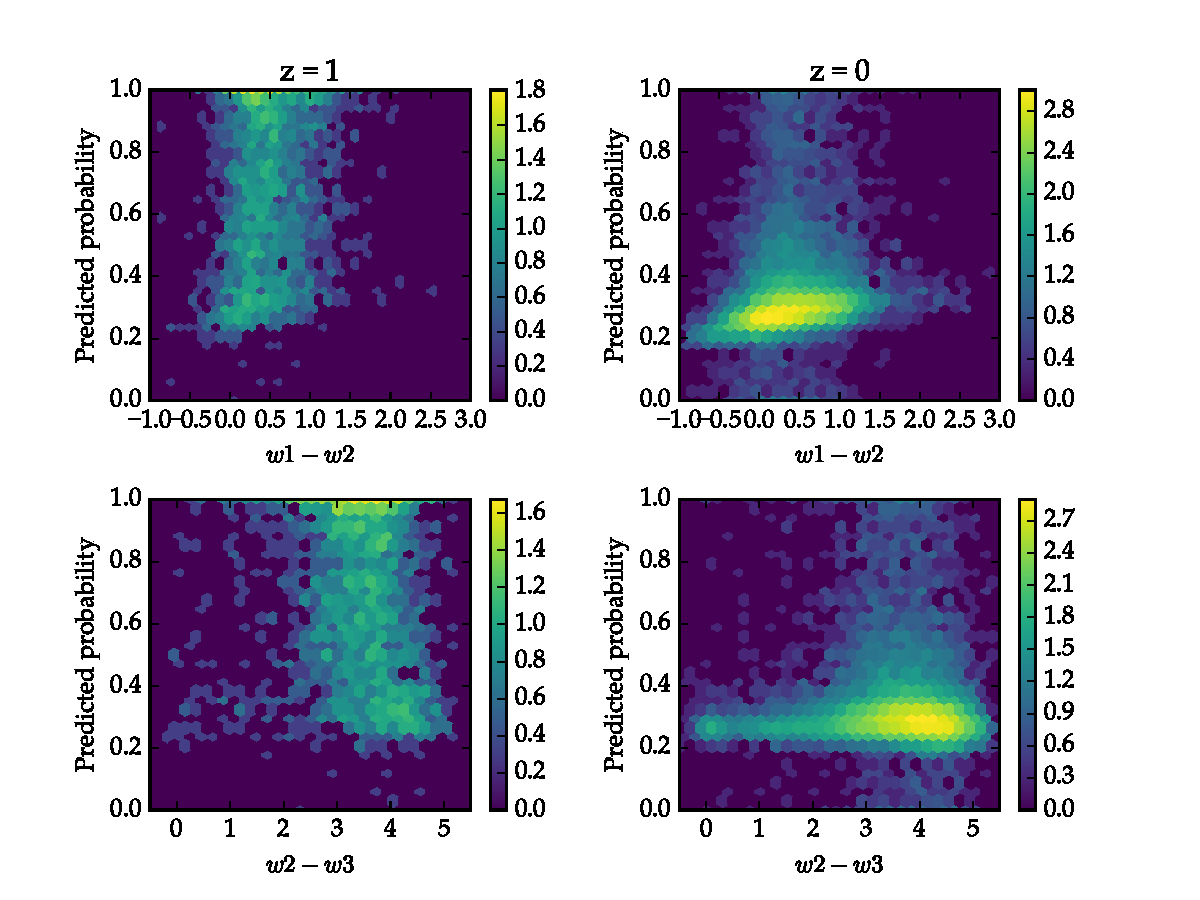
\includegraphics[width=\textwidth]{images/experiments/wise_colours}
      \caption{WISE magnitude difference features against predicted probability
        of a galaxy containing an AGN. Colours represent the logarithm of
        occurrences of instances in each cell.}
      \label{fig:wise-colours}
    \end{figure}

\section{Choosing a Binary Classifier}
\label{sec:binary-classifiers}
  
  \begin{figure}
    \centering
    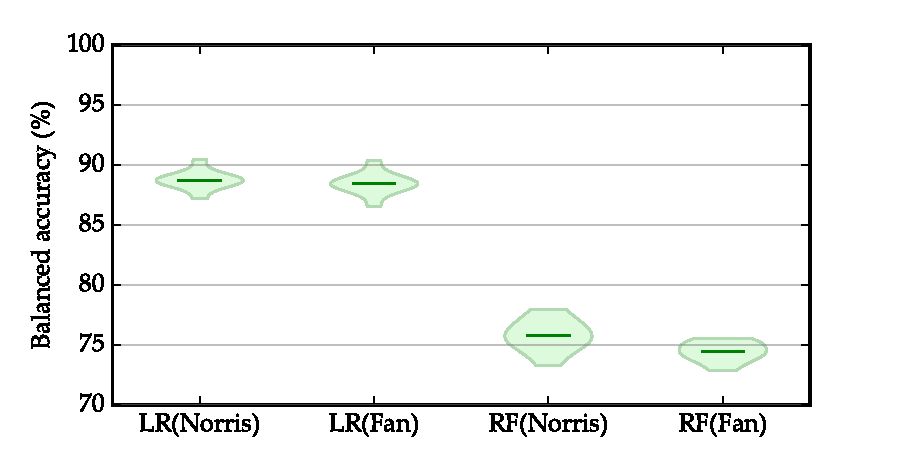
\includegraphics[width=\textwidth]{images/experiments/lr_rf}
    \caption{Comparison of logistic regression and random forests on the galaxy
      classification task, trained on the \citet{norris06} and \citet{fan15}
      label sets, and tested against the \citet{norris06} label set.}
  \end{figure}

  To compare the performance of logistic regression with random forests on the
  galaxy classification task, we performed the following experiment. We first
  generated five test sets of WISE objects. Then, using all other WISE objects
  as a training set, we trained a logistic regression classifier with $L2$
  regularisation for each test set, separately using labels from both
  \citet{norris06} and from \citet{fan15}. We then computed the balanced
  accuracy for each classifier. This was repeated for random forests, with each
  tree using $\sqrt{D}$ features.

  To generate the test sets, we first selected at random half of all ATLAS
  objects. We then added all WISE objects within $1'$ of a selected ATLAS object
  to the test set. This was repeated for each test set. The motivation for first
  selecting ATLAS objects rather than drawing WISE objects directly is that WISE
  objects have overlapping features, since radio features are taken from a patch
  of sky centred on each object, and WISE objects tend to be close together.
  Objects from the test sets were then removed at random until all test sets
  were the same size.

\section{Handling Crowd Labels}
\label{sec:rgz-crowd-labels}

  \begin{table}
    \centering
    \begin{tabular}{r|c}
      \textbf{Method(Training Set)} & \textbf{Mean Balanced Accuracy (\%)}\\\hline
      Raykar(Top-15-prolific) & $46.34 \pm 18.45$\\
      LR(Top-15-prolific-MV) & $51.98 \pm 3.87$\\
      Raykar(Top-15-accurate) & $86.43 \pm 0.10$\\
      LR(Top-15-accurate-MV) & $86.76 \pm 1.01$\\
      Raykar(Top-15-est-accurate) & $87.25 \pm 0.74$\\
      LR(Top-15-est-accurate-MV) & $87.25 \pm 0.90$\\
    \end{tabular}
    \caption{Comparison of logistic regression and \citeauthor{raykar10} on the
      galaxy classification task. These tests use only the $15$ best labellers,
      with ``best'' defined in three different ways: Total number of galaxies
      labelled (Top-15-prolific), balanced accuracy assessed against the
      \citeauthor{norris06} labels (Top-15-accurate), and balanced accuracy
      assessed against the Radio Galaxy Zoo majority vote (Top-15-est-accurate).
      Logistic regression (LR) is trained on the majority vote of the training
      labels; the \citeauthor{raykar10} method (Raykar) is trained on the labels
      themselves. Uncertainties are standard deviations across multiple test
      sets.}
    \label{tab:rgz-raykar}
  \end{table}

  \begin{figure}
    \centering
    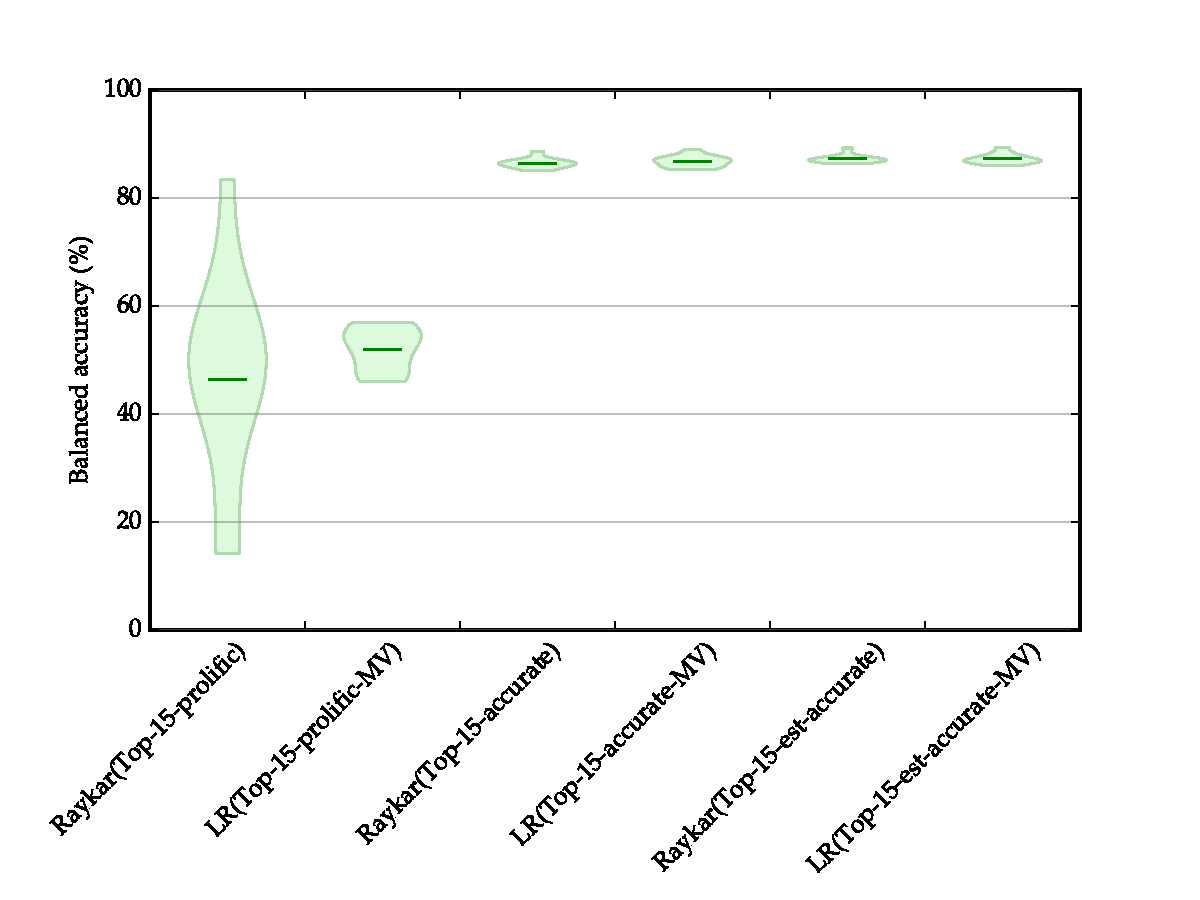
\includegraphics[width=\textwidth]{images/experiments/rgz_raykar}
    \caption{Comparison of logistic regression and \citeauthor{raykar10} on the
      galaxy classification task. Methods are denoted as in Table
      \ref{tab:rgz-raykar}. Spread along the vertical axis represents results
      across multiple test sets; the bar represents the mean.}
    \label{fig:rgz-raykar}
  \end{figure}

  While we want to train a classifier on the crowdsourced labels from the Radio
  Galaxy Zoo, it is unclear how we should aggregate the labels. Some methods for
  aggregation are described in Section \ref{sec:crowd-labels}. Which method will
  perform best on a dataset is dependent on the dataset itself, so we tested
  both variants of the \citeauthor{raykar10} algorithm and majority vote on the
  galaxy classification task.

  One key problem with the use of the \citeauthor{raykar10} algorithm is that it
  is very slow with large numbers of labellers. To mitigate this problem, we
  tested the algorithm on a subset of labellers, chosen by three different
  measures: the 10 labellers with the most labels, the 10 labellers with the
  highest balanced accuracy assessed against the \citeauthor{norris06} labels,
  and the 10 labellers with the highest balanced accuracy assessed against the
  majority vote of all labellers. While in practice on datasets such as EMU or
  FIRST there would be no equivalent to the \citeauthor{norris06} labels, we can
  treat this test as a ``best-case'' method. For each subset of labellers, the
  \citeauthor{raykar10} algorithm was tested against logistic regression trained
  on the majority vote of just these labellers. The results are shown in Figure
  \ref{fig:rgz-raykar} and Table \ref{tab:rgz-raykar}.

  With $T = 10$ labellers, the \citeauthor{raykar10} algorithm took $83 \pm 36$
  seconds to run. When the number of labellers was increased to $T = 15$, the
  \citeauthor{raykar10} algorithm took $152 \pm 115$ seconds to run. This helps
  to highlight how slow the algorithm becomes with increasing $T$.

  We also tried using all of the crowd labels directly with logistic regression,
  without aggregation. In principle, training logistic regression on such a
  label set may average over the conflicting labels and give reasonable results.
  This was not the case in practice; we found that this method resulted in a
  balanced accuracy of $50\%$ (i.e. random chance) as the classifier learned to
  always output 0.

\section{Galaxy Classification}
\label{sec:rgz-results}

  In this section, we present results using methods developed in this chapter.

  \subsection{Comparison of Methods}
  \label{sec:comparison-predictors}

    \begin{figure}
      \centering
      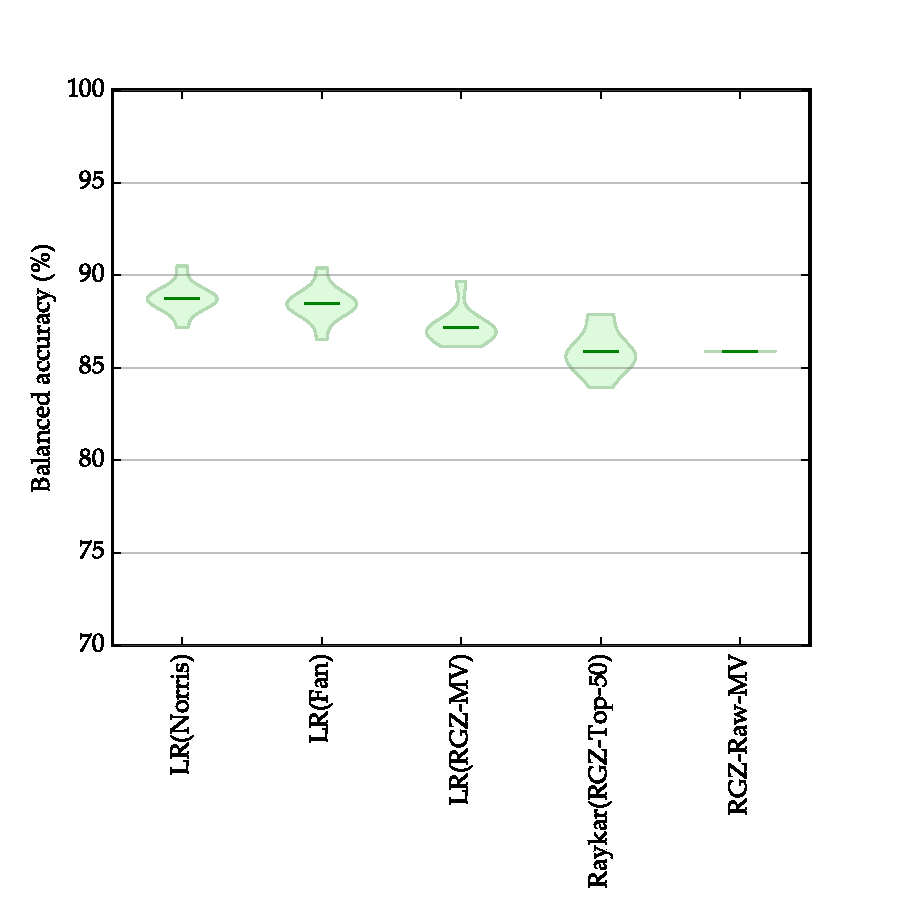
\includegraphics[width=\textwidth]{images/experiments/predictors.pdf}
      \caption{Performance of logistic regression and the \citeauthor{raykar10}
        algorithm on the galaxy classification task, trained on different sets of
        labels and tested on the galaxies where \citeauthor{norris06} and
        \citeauthor{fan15} labels agree. LR($Y$) indicates logistic regression
        trained on $Y$. RGZ-MV is the set of majority vote labels from the Radio
        Galaxy Zoo. RGZ-Raw-MV is the majority vote of all crowd labels and is
        included for comparison. Spread along the vertical axis represents
        results across multiple test sets; the bar represents the mean.}
      \label{fig:predictors}
    \end{figure}

    \begin{table}
      \centering
      \begin{tabular}{r|c}
        \textbf{Method(Training Set)} & \textbf{Mean Balanced Accuracy (\%)}\\\hline
        LR(Norris) & $88.74 \pm 0.77$\\
        LR(Fan) & $88.44 \pm 0.89$\\
        LR(RGZ-MV) & $87.17 \pm 0.90$\\
        Raykar(RGZ-Top-50) & $85.89 \pm 1.16$\\
        RGZ-Raw-MV & $85.89 \pm 0.00$\\
      \end{tabular}
      \caption{Performance of logistic regression and the \citeauthor{raykar10}
        algorithm on the galaxy classification task, as in Figure
        \ref{fig:predictors}. Uncertainties are standard deviations.}
      \label{tab:predictors}
    \end{table}

    \begin{table}
      \centering
      \begin{tabular}{l|ll}
          & $y = 0$  $(\%)$ & $y = 1$ $(\%)$ \\\hline
          $z = 0$ & $94.57 \pm 0.28$ & $5.43 \pm 0.28$\\
          $z = 1$ & $17.08 \pm 1.69$ & $82.92 \pm 1.69$
      \end{tabular}
      \caption{Confusion matrix for logistic regression trained on
        \citeauthor{norris06}.}
      \label{tab:cm-lr-norris}

      \vspace{10pt}

      \begin{tabular}{l|ll}
          & $y = 0$  $(\%)$ & $y = 1$ $(\%)$ \\\hline
          $z = 0$ & $95.93 \pm 0.26$ & $4.07 \pm 0.26$\\
          $z = 1$ & $19.03 \pm 1.94$ & $80.97 \pm 1.94$
      \end{tabular}
      \caption{Confusion matrix for logistic regression trained on
        \citeauthor{fan15}.}
      \label{tab:cm-lr-fan}

      \vspace{10pt}

      \begin{tabular}{l|ll}
          & $y = 0$  $(\%)$ & $y = 1$ $(\%)$ \\\hline
          $z = 0$ & $90.60 \pm 0.55$ & $9.40 \pm 0.55$\\
          $z = 1$ & $16.25 \pm 1.72$ & $83.75 \pm 1.72$\\
      \end{tabular}
      \caption{Confusion matrix for logistic regression trained on the Radio
        Galaxy Zoo majority vote.}
      \label{tab:cm-lr-rgz-mv}

      \vspace{10pt}

      \begin{tabular}{l|ll}
          & $y = 0$  $(\%)$ & $y = 1$ $(\%)$ \\\hline
          $z = 0$ & $87.88 \pm 1.34$ & $12.12 \pm 1.34$\\
          $z = 1$ & $16.09 \pm 1.42$ & $83.91 \pm 1.42$\\
      \end{tabular}
      \caption{Confusion matrix for the \citeauthor{raykar10} algorithm trained
        on the Radio Galaxy Zoo labels.}
      \label{tab:cm-raykar-rgz-raw}

      \vspace{10pt}

      \begin{tabular}{l|ll}
          & $y = 0$  $(\%)$ & $y = 1$ $(\%)$ \\\hline
          $z = 0$ & $92.47$ & $7.53$ \\
          $z = 1$ & $20.67$ & $79.33$ \\
      \end{tabular}
      \caption{Confusion matrix for the Radio Galaxy Majority vote.}
      \label{tab:cm-rgz-raw-mv}
    \end{table}

    We trained logistic regression classifiers on three training sets:
    \begin{itemize}
      \item the \citeauthor{norris06} labels,
      \item the \citeauthor{fan15} labels, and
      \item the Radio Galaxy Zoo majority vote.
    \end{itemize}
    We also trained the \citeauthor{raykar10} algorithm with the Radio Galaxy
    Zoo labels. Each volunteer was assigned a unique index and the algorithm was
    run with the best $T = 50$ labellers, computed against the Radio Galaxy Zoo
    majority vote. Finally, we compared the predictions of all classifiers to
    the Radio Galaxy Zoo majority vote. These results are plotted in Figure
    \ref{fig:predictors} and shown in Table \ref{tab:predictors}. The average
    confusion matrices normalised by class size are shown in Tables
    \ref{tab:cm-lr-norris} -- \ref{tab:cm-rgz-raw-mv}.

    The first observation we make is that logistic regression on our feature set
    does reasonably well. The \citeauthor{norris06} labels we are testing
    against are expected to have an error of around 9\%, so accuracies upwards
    of $85\%$ seem reasonable.

    The second observation we make is that logistic regression trained on the
    majority vote outperforms the \citeauthor{raykar10} classifier which makes
    use of the labels with no aggregation. This could occur for three reasons:
    We could have found a local minimum in the expectation-maximisation
    algorithm, using a subset of labellers instead of all labellers may lower
    performance, or the \citeauthor{raykar10} model may simply perform worse at
    this task than majority vote. Regardless, logistic regression and majority
    vote are very simple; these results indicate that perhaps we do not need a
    complicated algorithm for aggregating the Radio Galaxy Zoo labels.

    The third observation we make is that logistic regression trained on the
    Radio Galaxy Zoo labels performs comparably to logistic regression trained
    on the expert labels. This is a very good sign for citizen science,
    indicating that perhaps expert labels are not necessary, and supervised
    learning works just as effectively with crowd labels as with expert labels.
    However, it is hard to tell if this is a real effect; with our features set,
    logistic regression seems to have a maximum accuracy around $90\%$, and all
    classifiers attain accuracies close to this. It is possible that with better
    features, training on expert labels may give significantly better results
    than training on crowd labels.

    It is interesting to note that the \citeauthor{raykar10} classifier tends to
    overpredict positive labels when compared to the other methods. This may be
    a side-effect of the labeller model, or perhaps the best annotators are more
    ``over-eager'' and overpredict positive labels themselves.

    The final observation we make is that logistic regression trained on the
    Radio Galaxy Zoo majority vote outperforms the Radio Galaxy Zoo majority
    vote. This could be coincidence, or it could indicate some amount of noise
    reduction from applying logistic regression --- for example, our logistic
    regression model was trained with $L2$ regularisation, which could ``smooth
    over'' noise.

  \subsection{Raykar-estimated Labeller Accuracies}
  \label{sec:raykar-estimates-rgz}

    The \citeauthor{raykar10} algorithm estimates a labeller model parametrised
    by $\alpha$ and $\beta$ (Section \ref{sec:raykar}). In this section, we look
    at the estimated values of $\alpha$ and $\beta$ for the 50 best Radio Galaxy
    Zoo volunteers, and compare these to their ``true'' values.

    We computed the true $\alpha$ and true $\beta$ values for each labeller
    empirically, with $\alpha_t$ given by the true positive rate of labeller $t$
    and $\beta_t$ given by the true negative rate of labeller $t$. There were no
    labellers in the best 50 for whom these rates could not be calculated (i.e.
    the best 50 labellers had always labelled at least one positive and at least
    one negative galaxy).

    To assess the correlation between the true and predicted values of $\alpha$
    and $\beta$, we computed the Pearson and Spearman correlation coefficients
    between the true and predicted values using \texttt{scipy.stats}
    \citep{scipy}.

    According to the Pearson correlation coefficient, the true and predicted
    values of $\alpha$ were weakly correlated, with $r = 0.11$ and $p = 0.01$;
    the true and predicted values of $\beta$ were not, with $r = -0.01$ and $p =
    0.75$. According to the Spearman correlation coefficient, the true and
    predicted values of $\alpha$ were weakly correlated, with $r = 0.32$ and $p
    = 0.00$; the true and predicted values of $\beta$ were also correlated, with
    $r = 0.21$ and $p = 0.00$.

    We make two notes on these results. First, the Pearson correlation
    coefficient assumes that the values being tested are normally distributed,
    which the $\alpha$ and $\beta$ values are not. Second, \texttt{scipy.stats}
    comments that the output $p$ values are ``not entirely reliable'' though the
    reliability increases with larger datasets.

    These results may imply that the labeller model does not accurately describe
    the Radio Galaxy Zoo volunteers. It is possible that a data-dependent model
    like that proposed by \citeauthor{yan10} may provide a better model, but due
    to the difficulty and slow speed of trialling labeller models with many
    parameters, we do not further investigate this problem in this thesis.

\section{Conclusion and Future Work}
\label{sec:cross-identification-conclusion-future-work}
  
  In this chapter, we cast the radio cross-identification problem as a
  classification problem, and developed a classifier to solve it. We represented
  galaxies as a combination of astronomical features and features extracted from
  radio images. We used logistic regression on three different sets of training
  labels and compared the performance of these to the \citeauthor{raykar10}
  crowd learning model, finding that logistic regression outperformed the
  \citeauthor{raykar10} model. Additionally, we found that training logistic
  regression on non-expert labels results in performance comparable to training
  on experts, showing that efforts to crowd-label scientific data may generalise
  just as well as expert labels when machine learning is applied.

  % This is a good sign for citizen science, as it indicates that efforts to
  % crowd-label scientific data may generalise just as well as expert labels
  % when machine learning is applied.

  For the remainder of this section, we will briefly discuss the problems in our
  method and highlight some avenues for future work.

  A clear place that our methods could be improved is in our feature selection.
  Other studies, such as those by \citet{proctor06} and \citet{fan15}, have made
  use of hand-selected features for radio classification. These could possibly
  be incorporated into the galaxy feature set (though as these hand-selected
  features are features of radio objects rather than of galaxies, doing so may
  be non-trivial). We may also be able to make use of information from
  catalogues at wavelengths other than infrared. In particular, we may be able
  to make use of information from the ATLAS catalogue, which includes values
  such as the rotation of extended radio sources.

  Our approach to image feature extraction was very simple. We did not fully
  investigate all of the many different possible architectures for a
  convolutional neural network, and it is possible that better networks exist
  for radio data. Improvements could be made in our parameters (filter size,
  pooling size, etc.) and in our network topology (number of layers, structure
  of layers, etc.). We could also rescale and rotate training images to ensure
  rotational and scale invariance in our convolutional features. This was
  successfully applied to galaxy morphology prediction using Galaxy Zoo data by
  \citet{dieleman15}, though we note that these results were obtained in optical
  wavelengths where resolution is higher and images are clearer.

  There may be useful information to extract from the infrared images,
  particularly in higher resolution surveys like SWIRE. As preliminary results
  suggested there were no strong features in the infrared images, we ignored
  them for this work, but this was only a passing investigation of infrared
  features. One possible avenue for investigation is to include infrared
  \emph{and} radio images as different channels in our convolutional neural
  network. These networks are capable of supporting multiple colour channels and
  radio and infrared are effectively colour channels. This would also allow the
  full use of multi-wavelength data from telescopes like WISE and Spitzer.

  An obvious drawback of our approach to object localisation is that
  infrared-faint radio objects are not able to be classified. There is no clear
  way around this without dramatically increasing the running time of our
  method. A possible option is to allow the classifier to output an
  ``undecided'' choice when there is no clear infrared counterpart to a radio
  object. These radio objects could then be investigated by hand, or distributed
  to a different algorithm.

  We note that the \citeauthor{raykar10} model performed relatively poorly on
  the galaxy classification task. In Section \ref{sec:raykar-estimates-rgz} we
  suggested some reasons that this might be the case. Further investigation of
  these results is needed, in particular, whether using a different labeller
  model would improve results. One such model would be the \citeauthor{yan10}
  model, but as we noted in Section \ref{sec:yan} this is very slow and seems to
  yield mediocre results for large numbers of annotators. Careful analysis of
  the Radio Galaxy Zoo data set may reveal ``clusters'' where labellers perform
  better or worse, and these patterns could be exploited to develop a labeller
  model that requires less parameters than simply using all features.

  Finally, in this work we only investigated the cross-identification problem on
  a per-object basis. We did not investigate the problem of determining which
  radio objects are associated with each other, e.g. detecting when two radio
  objects are simply two jets of the same object. This is potentially a much
  harder problem than cross-identification, yet it is important for astronomy.
  One possible approach is to use a classifier like we have developed, use this
  to identify galaxies that may contain AGNs, and then search around those
  galaxies for radio objects. This is similar to the approach taken by
  \citet{fan15}, though their algorithm was applied across the entirety of the
  CDFS field.
